\input{text/diss}
\begin{document}
\def\labauthors{Есюнин Д.В., Есюнин М.В.}
\def\labgroup{440}
\def\labnumber{1}
\def\labtheme{Исследование акустического поля в однородной среде с плоской границей}
%\def\department{Кафедра электроники и квантовой радиофизики}
\input{text/titlepage}
\newpage
\renewcommand{\phi}{\varphi}
\renewcommand{\div}{\text{div}}
\renewcommand{\grad}{\text{grad}}

\paragraph{Цель работы:}
Цель работы: исследование пространственного распределения звукового поля источника, находящегося в однородной среде вблизи гладкой поверхности раздела воздух-вода.
Приборы и оборудование: ультразвуковая экспериментальная установка, представляющая собой устройство для излучения и приема акустических импульсов, осциллограф.

\section{Теоретическая часть}
Колебательное движение в сжимаемой жидкости называется звуковыми волнами. Звуковая волна может быть полностью описана следующими уравнениями:
\begin{equation}
	\frac{\partial\vec{v}}{\partial t}+\frac{\nabla p'}{\rho_0}=0
	\label{eq:1}
\end{equation}

\begin{equation}
\frac{\partial p'}{\partial t}+\rho_0 \frac{\partial p}{\partial p_0}\div\vec{v}=0
\label{eq:2}
\end{equation}
 $\vec{v}=\grad\phi$, $\phi$ - потенциал скорости, который удовлетворяет волновому уравнению:
 
 \begin{equation}
 \frac{\partial^2 \phi}{\partial t^2}-c^2 \nabla\phi=0
 \label{eq:3}
 \end{equation}
 где $\displaystyle c=\sqrt{\left(\frac{\partial p}{\partial \rho}\right)_s}$ - скорость звука
 
Важным случаем волн являются монохроматические волны $\phi=\Re{\phi_0(x,y,z)e^{-i\omega t}}$ .
$\phi_0$ удовлетворяет уравнению Гельмгольца $\nabla \phi_0+k^2\phi_0=0$.
Два простейших решения этого уравнения:

А) Сферическая волна  $\displaystyle \phi=\frac{-V_0}{4\pi R}\exp(ikR)$;

Б) Плоская волна $\phi=A\exp(i\vec{k}\vec{r})$

\newpage
\section{Экспериментальная часть}
\paragraph{Описание установки}

\subsection{Диаграмма направленности излучателя}
Для снятия диаграммы направленности, излучатель был погружен в воду на глубину 15 см. Приемный щуп был расположен на той же глубине. Измерения проводились в зоне Фраунгофера при условиях полного разделения отраженного и приемного по времени прихода. 

Для того, чтобы убедиться, что все условия были выполнены, оценим значение расстояния между приемным и передающим расстоянием с учетом выполнения неравенства $p>>1$, где $\displaystyle p=\sqrt{\frac{\lambda r}{D}}$ - волновой параметр, $\lambda=1.5 \text{ мм}$ - длина волны, $D=10 \text{ мм}$ - характерный размер излучателя. Тогда 
\begin{equation}
r>>\frac{D^2}{\lambda}\approx 6 \text{ см}
\label{eq:pr1}
\end{equation}


Второе - прямой и отраженный импульс должны полностью разделяться по времени прихода. Чтобы это условие выполнялось,
необходимо, чтобы время прихода отраженного импульса $t_2$ было больше, чем величина $t_1+\tau$, где $t_1$ - время
прихода прямого импульса, а $\tau$ - длительность импульса.
\begin{figure}[h!]
	\centering
	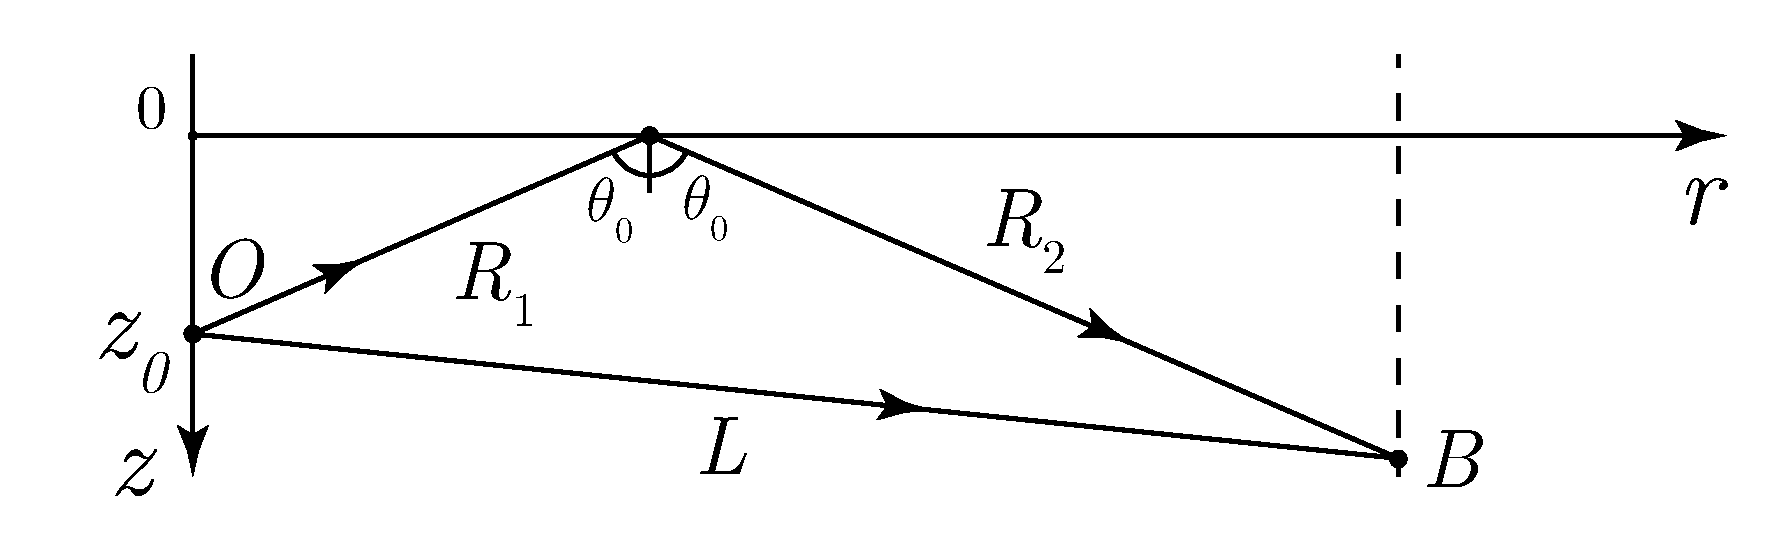
\includegraphics[width =0.7\linewidth]{fig/scheme2.pdf}
	\caption{Схема к расчету расстояния между источником и приемником}
	\label{fig:expt:scheme2}
\end{figure}

\begin{equation}
	t_2 > t_1 + \tau, \quad t_1 = \frac{L}{c}, t_2 = \frac{R_1+R_2}{c}
\end{equation}
В достаточно грубом приближении, считая $L \sim 1$ м, а $R_1+R_2 \sim 1.5$ м, можно получить:
\begin{equation}
	\tau < \frac{R_1+R_2-L}{c} \simeq \frac{0.5}{1500} = 3 \cdot 10^{-4} \text{ с}
\end{equation}
\begin{equation}
	\tau < 300 \text{ мкс}
	\label{eq:time_cond}
\end{equation}
В работе использовалось $\tau = 100$ мкс, что удовлетворяет условию \eqref{eq:time_cond}.

Отнормированная диаграмма направленности излучателя, а также расчитанная теоретически в приближении плоского диска
приведены на рис. \ref{fig:direct1}. В качестве теоретической характеристики использовалась характеристика круглой
плоской антенны с диаметром $d$:
\begin{equation}
	b(\theta) = \frac{2 J_1[ \frac{\pi d}{\lambda} \cos \theta ]}{\frac{\pi d}{\lambda} \cos \theta },
	\label{eq:bessel_disk}
\end{equation}
где $J_1$ - функция Бесселя первого порядка.
\begin{figure}[H]
	\centering
	\includegraphics[width=\linewidth]{pic/diag1.png}
	\caption{Нормированная диаграмма направленности излучателя}
	\label{fig:direct1}
\end{figure}
\begin{figure}[H]
	\centering
	\includegraphics[width=\linewidth]{pic/diag2.png}
	\caption{Нормированная диаграмма направленности излучателя}
	\label{fig:direct2}
\end{figure}

\subsection{Исследование распределения звукового давления}
\begin{figure}[h!]
	\centering
	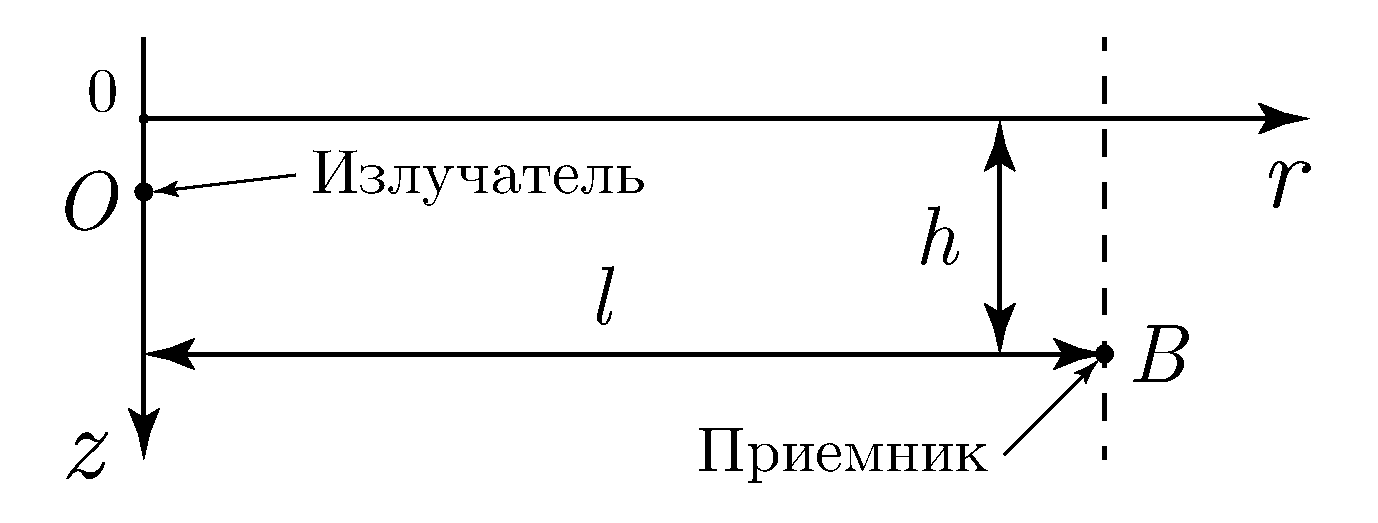
\includegraphics[width =\linewidth]{fig/scheme3.pdf}
	\caption{Схема постановки эксперимента}
	\label{fig:expt:scheme3}
\end{figure}
Излучатель был расположен на глубине $\sim 3$ см, чтобы полностью быть погруженным в воду.
С помощью приемного щупа было произведено исследовано распределение звукового давления в ванне, были произведены три
продольных разреза на глубинах $h = 1,2,3$ см, и три вертикальных среза на расстояниях $l=60,90,120$ см.

Теоретическое значение для модуля амплитуды суммарного давления рассчитывалось по формуле \eqref{eq:pressure}:
\begin{equation}
	|P(h,R)| = \sqrt{ \frac{1}{R^2} + \frac{1}{R_1^2} - \frac{2}{R_1 R} \cos k \Delta R },\quad \Delta R = R-R_1,
	\label{eq:pressure}
\end{equation}
где $R^2 = l^2+(h-z_0)^2$, а $R_1^2 = l^2 + (h+z_0)^2$, $k$ - волновое число.

% Table generated by Excel2LaTeX from sheet 'Лист1'
\begin{table}[htbp]
	\centering
%	\caption{Add caption}
	\begin{tabular}{|r|r|r|r|r|r|}
		\toprule
		\multicolumn{2}{|c|}{$h$ = 1 см} & \multicolumn{2}{c|}{$h$ = 2 см} & \multicolumn{2}{c|}{$h$ = 3 см} \\
		\midrule
		\multicolumn{1}{|l|}{$z$, см} & \multicolumn{1}{l|}{$2A$, В} & \multicolumn{1}{l|}{$z$, см} & \multicolumn{1}{l|}{$2A$, В} & \multicolumn{1}{l|}{$z$, см} & \multicolumn{1}{l|}{$2A$, В} \\
		\midrule
		1.8   & 0.8   & 1.4   & 2.36  & 1     & 0.76 \\
		\midrule
		5.3   & 2.48  & 3.1   & 0.92  & 1.7   & 1.8 \\
		\midrule
		8.8   & 0.28  & 4.5   & 2.24  & 2.9   & 0.86 \\
		\midrule
		16    & 1.72  & 6.3   & 0.36  & 3.8   & 1.6 \\
		\midrule
		25.5  & 0.2   & 9     & 2.12  & 5.2   & 0.52 \\
		\midrule
		47.5  & 0.68  & 10.7  & 0.24  & 6.3   & 1.64 \\
		\midrule
		111   & 0.28  & 14.2  & 1.88  & 7.6   & 0.2 \\
		\midrule
		16    & 1.72  & 18.3  & 0.32  & 9.5   & 1.52 \\
		\midrule
		25.5  & 0.2   & 24    & 1.44  & 11.3  & 0.2 \\
		\midrule
		47.5  & 0.68  & 31.6  & 0.24  & 13.7  & 1.52 \\
		\midrule
		111   & 0.28  & 45.7  & 0.8   & 16.3  & 0.36 \\
		\midrule
		&       & 62    & 0.12  & 19.8  & 1.52 \\
		\midrule
		&       & 105   & 0.44  & 25.5  & 0.4 \\
		\midrule
		&       &       &       & 27.8  & 1.28 \\
		\midrule
		&       &       &       & 34.2  & 0.28 \\
		\midrule
		&       &       &       & 41.5  & 0.84 \\
		\midrule
		&       &       &       & 54.5  & 0.2 \\
		\midrule
		&       &       &       & 69    & 0.56 \\
		\midrule
		&       &       &       & 101   & 0.16 \\
		\bottomrule
	\end{tabular}%
%	\label{tab:addlabel}%
\end{table}%

\begin{figure}[H]
	\centering
	\includegraphics[width =0.75\linewidth]{pic/z2_1}
	\caption{Амплитуды максимумов и минимумов при продольном срезе, на расстоянии $h=1$ см}
	\label{fig:task21}
\end{figure}

\begin{figure}[H]
	\centering
	\includegraphics[width =0.75\linewidth]{pic/z2_2}
	\caption{Амплитуды максимумов и минимумов при продольном срезе, на расстоянии $h=2$ см}
	\label{fig:task22}
\end{figure}

\begin{figure}[H]
	\centering
	\includegraphics[width =0.75\linewidth]{pic/z2_3}
	\caption{Амплитуды максимумов и минимумов при продольном срезе, на расстоянии $h=3$ см}
	\label{fig:task23}
\end{figure}

% Table generated by Excel2LaTeX from sheet 'Лист1'
\begin{table}[htbp]
	\centering
%	\caption{Add caption}
	\begin{tabular}{|r|r|r|r|r|r|}
		\toprule
		\multicolumn{2}{|c|}{$z$ = 60 см} & \multicolumn{2}{c|}{$z$ = 90 см} & \multicolumn{2}{c|}{$z$ = 120 см} \\
		\midrule
		\multicolumn{1}{|l|}{$h$, см} & \multicolumn{1}{l|}{$2A$, В} & \multicolumn{1}{l|}{$h$, см} & \multicolumn{1}{l|}{$2A$, В} & \multicolumn{1}{l|}{$h$, см} & \multicolumn{1}{l|}{$2A$, В} \\
		\midrule
		12.4  & 0.2   & 26.4  & 0.056 & 14    & 0.328 \\
		\midrule
		13.2  & 0.72  & 25.5  & 0.616 & 15.5  & 0.02 \\
		\midrule
		13.7  & 0.2   & 24.6  & 0.088 & 16.5  & 0.332 \\
		\midrule
		14.4  & 0.8   & 23.9  & 0.584 & 17.7  & 0.04 \\
		\midrule
		14.9  & 0.2   & 23    & 0.104 & 18.8  & 0.35 \\
		\midrule
		15.5  & 0.704 & 22.1  & 0.56  & 19.8  & 0.045 \\
		\midrule
		15.9  & 0.15  & 21.2  & 0.112 & 20.8  & 0.368 \\
		\midrule
		16.5  & 0.79  & 20.6  & 0.512 & 22    & 0.052 \\
		\midrule
		17    & 0.17  & 19.5  & 0.112 & 23.1  & 0.04 \\
		\midrule
		17.6  & 0.8   & 18.7  & 0.504 & 25.5  & 0.432 \\
		\midrule
		18.2  & 0.18  & 17.9  & 0.088 & 26.6  & 0.056 \\
		\midrule
		18.7  & 0.83  & 17    & 0.464 & 27.7  & 0.448 \\
		\midrule
		19.3  & 0.19  & 16.2  & 0.08  &       &  \\
		\midrule
		19.9  & 0.856 & 15.4  & 0.456 &       &  \\
		\midrule
		20.4  & 0.16  & 14.6  & 0.02  &       &  \\
		\midrule
		21    & 0.856 & 13.6  & 0.476 &       &  \\
		\midrule
		21.7  & 0.088 &       &       &       &  \\
		\midrule
		22.5  & 0.808 &       &       &       &  \\
		\midrule
		22.9  & 0.064 &       &       &       &  \\
		\midrule
		23.4  & 0.8   &       &       &       &  \\
		\midrule
		24    & 0.112 &       &       &       &  \\
		\midrule
		24.6  & 0.768 &       &       &       &  \\
		\midrule
		25.2  & 0.144 &       &       &       &  \\
		\midrule
		25.8  & 0.736 &       &       &       &  \\
		\midrule
		26.4  & 0.16  &       &       &       &  \\
		\midrule
		26.9  & 0.648 &       &       &       &  \\
		\midrule
		27.6  & 0.2   &       &       &       &  \\
		\bottomrule
	\end{tabular}%
%	\label{tab:addlabel}%
\end{table}%


\begin{figure}[H]
	\centering
	\includegraphics[width =0.75\linewidth]{pic/z3_1}
	\caption{Амплитуды максимумов и минимумов при вертикальном срезе, на расстоянии $l=60$ см}
	\label{fig:task31}
\end{figure}

\begin{figure}[H]
	\centering
	\includegraphics[width =0.75\linewidth]{pic/z3_2}
	\caption{Амплитуды максимумов и минимумов при вертикальном срезе, на расстоянии $l=90$ см}
	\label{fig:task32}
\end{figure}

\begin{figure}[H]
	\centering
	\includegraphics[width =0.6\linewidth]{pic/z3_3}
	\caption{Амплитуды максимумов и минимумов при вертикальном срезе, на расстоянии $l=120$ см}
	\label{fig:task33}
\end{figure}

Если учесть диаграмму направленности излучателя, то выражение для модуля амплитуды суммарного давления видоизменится.
\begin{equation}
|P(h,R)| = \sqrt{ \frac{b^2(\theta_2)}{R^2} + \frac{b^2(\theta_0)}{R_1^2} - \frac{2b(\theta_2)b(\theta_0)}{R_1 R} \cos k \Delta R },\quad \Delta R = R-R_1,
\label{eq:pressure2}
\end{equation}
где $b(\theta)$ - диаграмма направленности круглой плоской антенны, которая задается выражением \eqref{eq:bessel_disk}. Углы $\theta_2$ и $\theta_0$ определяются следующим образом $\displaystyle \cos\theta_2=\frac{z-h}{R}$, $\displaystyle \cos\theta_0=\frac{z+h}{R}$

В таком случае, распределение давления по глубине на различных расстояниях представлено ниже. 
\begin{figure}[H]
	\centering
	\includegraphics[width =0.6\linewidth]{pic/z3_1th}
	\caption{Амплитуды максимумов и минимумов при вертикальном срезе, на расстоянии $l=60$ см}
	\label{fig:task31th}
\end{figure}

\begin{figure}[H]
	\centering
	\includegraphics[width =0.7\linewidth]{pic/z3_2th}
	\caption{Амплитуды максимумов и минимумов при вертикальном срезе, на расстоянии $l=90$ см}
	\label{fig:task32th}
\end{figure}

\begin{figure}[H]
	\centering
	\includegraphics[width =0.7\linewidth]{pic/z3_3th}
	\caption{Амплитуды максимумов и минимумов при вертикальном срезе, на расстоянии $l=120$ см}
	\label{fig:task33th}
\end{figure}

\section{Вывод}
Исследовали пространственного распределения звукового поля источника, находящегося в однородной среде вблизи гладкой поверхности раздела воздух-вода.
\end{document}
